Optical flow\textsuperscript{\cite{optical_flow}} คือการแปลงการเคลื่อนที่ของวัตถุในระหว่างสองภาพซึ่งอาจจะเกิดจากการเคลื่อนที่ของวัตถุหรือตัวกล้องออกมาในรูปแบบของเวกเตอร์ 2 มิติ 
โดยที่เวกเตอร์แต่ละตัวจะแสดงถึงทิศทางการเคลื่อนที่ของวัตถุหรือบุคคลระหว่างภาพดังรูปที่ \ref{fig:vector_optical}

\begin{figure}[!ht]
	\centering
	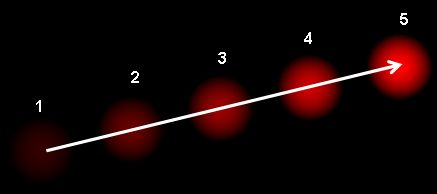
\includegraphics[width=1\textwidth]{chapter2/images/vector_optical.png}
		\caption[ตัวอย่าง optical flow ของการเคลื่อนที่ของลูกบอล]{ตัวอย่าง optical flow ของการเคลื่อนที่ของลูกบอล\textsuperscript{\cite{optical_flow}}}
    	\label{fig:vector_optical}
\end{figure}

จากรูปที่ \ref{fig:vector_optical} แสดงให้เห็นถึงการเคลื่อนที่ของลูกบอลในภาพที่ต่อเนื่องกัน 5 ภาพ โดยที่ลูกศรจะแสดงถึงทิศทางการเคลื่อนที่ของเวกเตอร์

การทำงานของ optical flow อยู่บนสมมติฐาน 2 ประการได้แก่
\begin{enumerate}
	\setlength\itemsep{-0.25em}
	\item ความเข้มพิกเซลของวัตถุจะไม่เปลี่ยนแปลงระหว่างภาพที่ต่อเนื่องกัน
	\item พิกเซลที่อยู่ใกล้กันจะมีลักษณะการเคลื่อนไหวที่คล้ายกัน
\end{enumerate}

เมื่อพิจารณาพิกเซล $I(x,y,t)$ จากภาพแรกจะเคลื่อนไหวเป็นระยะทาง $(dx,dy)$ ไปยังภาพต่อไปหลังจากเวลาผ่านไปแล้ว $dt$ ดังนั้นเนื่องจากพิกเซลเหล่านี้เหมือนกัน 
และความเข้มไม่มีการเปลี่ยนแปลง จึงทำให้พูดได้ว่า

\begin{equation}
I(x,y,t) = I(x + dx, y + dy, t + dt)
\end{equation}
โดยที่
\begin{conditions}
I 		&	พิกเซลจากภายในภาพ				\\
x 		&	ตำแหน่งของพิกเซลในแกน x 		\\
dx		&	ระยะทางที่เคลื่อนที่ในแกน x 			\\
y		&	ตำแหน่งของพิกเซลในแกน y 		\\
dy		&	ระยะทางที่เคลื่อนที่ในแกน y 			\\
t 		&	เวลา							\\
dt		&	ระยะเวลาที่เปลี่ยนไประหว่างภาพ
\end{conditions}

จากนั้นใช้การประมาณค่าของ taylor series ทางฝั่งขวามือ และลบค่า common term แล้วหารด้วย $dt$ เพื่อให้ได้สมการดังต่อไปนี้
\begin{equation}
f_{x}u + f_{y}v + f_{t}
\end{equation}
\begin{equation}
f_{x} = \frac{\delta f}{\delta x} ; f_{y} = \frac{\delta f}{\delta y}
\end{equation}
\begin{equation}
u = \frac{\delta x}{\delta t} ; v = \frac{\delta y}{\delta t}
\end{equation}
โดยที่
\begin{conditions}
f_{x}		&	เกรเดียน (gradient) ในแกน x 		\\
f_{y}		&	เกรเดียนในแกน y				\\
f_{t}		&	เกรเดียนของเวลา				\\
u 		&	เวกเตอร์การเคลื่อนที่ของแกน x 	\\
v		&	เวกเตอร์การเคลื่อนที่ของแกน y	\\
\end{conditions}
สมการข้างบนเรียกว่าสมการ optical flow จากสมการทำให้สามารถหา $f_{x}$ และ $f_{y}$ เป็นเกรเดียนของภาพในแกน x และแกน y ตามลำดับ และ $f_{t}$ เป็นเกรเดียนของเวลา 
แต่ $u$ กับ $v$ เป็นตัวแปรที่ไม่ทราบ ทำให้สมการนี้ไม่สามารถแก้ไขด้วยมีตัวแปรที่ไม่ทราบถึง 2 ตัว จึงมีการนำวิธีการต่างๆเข้ามาใช้ในการแก้ปัญหานี้
โดยวิธีการที่นำเข้ามาใช้ในการแก้ปัญหา คือ อัลกอริทึมของ Gunner Farneback\textsuperscript{\cite{farneback2003two}} ซึ่งใช้หลักการ polynomial expansion เป็นการประมาณค่าของพื้นที่บางส่วนที่อยู่รอบ ๆ ของแต่ละพิกเซลด้วยสมการพหุนาม
โดย optical flow เป็นหนึ่งในวิธีการสกัดข้อมูลการเคลื่อนไหวของวิดีโอออกมาเพื่อใช้เป็นข้อมูลในการสร้างโมเดลปัญญาประดิษฐ์สำหรับจำแนกการกระทำหรือเหตุการณ์ในวิดีโอ